\chapter{Θεωρία}
\section{Μέση τετραγωνική μετατόπιση}
Μία από τις μεταβλητές τις οποίες θα υπολογίσουμε στα πειράματά μας είναι η μέση τετραγωνική μετατόπιση ενός τυχαίου περιπάτου. 
Ο απλούστερος τυχαίος περίπατος είναι μονοδιάστατος. Έστω μία μαύρη τελεία στην γραμμή των ακεραίων η οποία ξεκινάει από το κέντρο. 
\begin{figure}[H]
\begin{center}
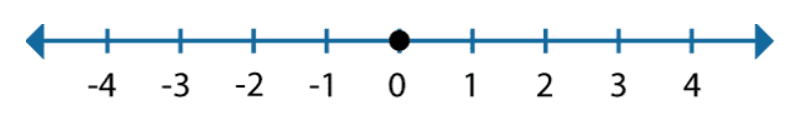
\includegraphics[scale=0.9]{figures/TheoryRW1.png}
\end{center}
\end{figure}
\noindent
Η τελεία ξεκινά να κινείτε είτε αριστερά είτε δεξιά με ίση πιθανότητα 1/2. Ας καλέσουμε το πρώτο βήμα $a_1$, το δεύτερο βήμα $a_2$ κ.ο.κ. Κάθε $a$ έχει είτε την τιμή -1 (κίνηση αριστερά), είτε την τιμή +1 (κίνηση δεξιά).
Για παράδειγμα: 
\begin{figure}[H]
\begin{center}
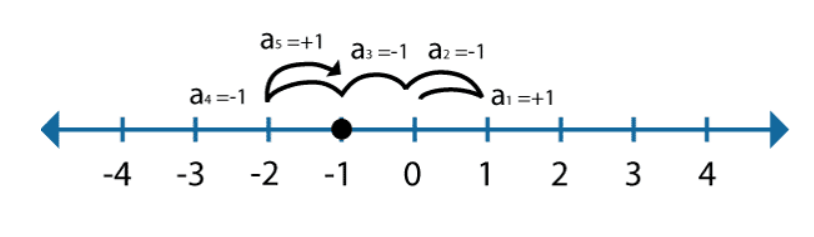
\includegraphics[scale=0.9]{figures/TheoryRW2.png}
\end{center}
\end{figure}
\noindent
Ας υπολογίσουμε την μέση τετραγωνική απόσταση ενός τυχαίου περιπάτου $N$ βημάτων:
\begin{equation}
\begin{aligned}
&\left\langle d^{2}\right\rangle=\left\langle\left(a_{1}+a_{2}+a_{3}+\ldots+a_{N}\right)^{2}\right\rangle=\left\langle\left(a_{1}+a_{2}+a_{3}+\ldots+a_{N}\right)\left(a_{1}+a_{2}+a_{3}+\ldots+a_{N}\right)\right\rangle\\
&=\left(\left\langle a_{1}^{2}\right\rangle+\left\langle a_{2}^{2}\right\rangle+\left\langle a_{3}^{2}\right\rangle+\ldots+\left\langle a_{N}^{2}\right\rangle\right)+2\left(\left\langle a_{1} a_{2}\right\rangle+\left\langle a_{1} a_{3}\right\rangle+\ldots\left\langle a_{2} a_{N}\right\rangle+\ldots\right)
\end{aligned}
\label{msd}
\end{equation}
Είναι προφανές ότι τα $a_i^2$ με $i=1,2...N$, είναι πάντα ίσα με 1, μιας και η μόνες πιθανές τιμές των $a_i$ είναι -1 και 1. Επομένως, ο πρώτος όρος της \eqref{msd} δίνει $(1+1....+1) = Ν$. Ο δεύτερος όρος έχει το άθροισμα όλων των μέσων όρων των γινομένων διαφορετικών βημάτων, δηλαδή των $\langle a_i a_j \rangle$ με $i\neq j$.
Οι πιθανές τιμές του των γινομένων είναι:
\begin{equation}
\begin{array}{rcc}
a_{i} & a_{j} & a_{i} a_{j} \\
1 & 1 & 1 \\
1 & -1 & -1 \\
-1 & 1 & -1 \\
-1 & -1 & 1
\end{array}
\end{equation}
Δηλαδή έχουμε -1 με πιθανότητα 1/2 και 1 με πιθανότητα 1/2. Προφανώς ο μέσος όρος αυτών των τιμών είναι 0. Συνεπώς, ο δεύτερος όρος δίνει $2(0+0...+0)$. Άρα τελικά, η αναμενόμενη τετραγωνική μετατόπιση ενός τυχαίου περιπάτου σε μία διάσταση, είναι ίση με τον αριθμό $Ν$ των βημάτων του τυχαίου περιπάτου, εφόσον {\en step = 1}.

Μπορεί κανείς εύκολα με την ίδια λογική, να αποδείξει το ίδιο αποτέλεσμα για ένα δισδιάστατο τυχαίο περίπατο. Έχουμε τώρα δύο κάθετους μεταξύ τους άξονες $\mathbb{Z}$, δηλαδή ένα πλέγμα, στο οποίο τώρα η μετατόπιση υπολογίζεται με το πυθαγώρειο θεώρημα (μπλε γραμμή).

\begin{figure}[H]
\begin{center}
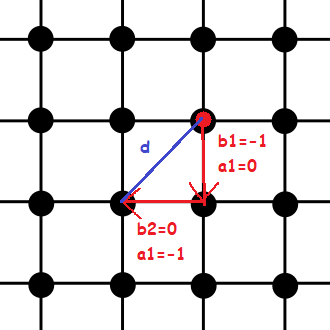
\includegraphics[scale=1.1]{figures/TheoryRW3.png}
\end{center}
\end{figure}

Το σωματίδιο ( κόκκινο ) έχει 1/4 πιθανότητα να κινηθεί σε μία από τις 4 κατευθύνσεις, άρα έχει 1/4 να κάνει +1, 1/4 να κάνει -1, και 1/2 να μην κινηθεί. Επομένως, σε αυτή την περίπτωση αν ονομάσουμε $x$ και $y$ τις αποστάσεις που διένυσε ανά άξονα, τότε:  
\begin{equation}
\left\langle d^{2}\right\rangle=
\left\langle x^{2} + y^{2} \right\rangle
=\left\langle x^{2}\right\rangle + \left\langle y^{2}\right\rangle
\label{distanced}
\end{equation}
Είναι προφανές ότι $\left\langle x^{2}\right\rangle$ = $\left\langle y^{2}\right\rangle$ αφού πρόκειται για ανεξάρτητους άξονες στους οποίους στατιστικά συναντάμε ακριβώς την ίδια συμπεριφορά. 
Άρα: 
\begin{equation}
\left\langle y^{2}\right\rangle=\left(\left\langle b_{1}^{2}\right\rangle+\left\langle b_{2}^{2}\right\rangle+\left\langle b_{3}^{2}\right\rangle+\ldots+\left\langle b_{N}^{2}\right\rangle\right)+2\left(\left\langle b_{1} b_{2}\right\rangle+\left\langle b_{1} b_{3}\right\rangle+\ldots\left\langle b_{2} b_{N}\right\rangle+\ldots\right) 
\label{eqy}
\end{equation}
Για τον μέσο όρου του τετραγώνου γνωρίζουμε από τα παραπάνω ότι έχουμε 1/2 πιθανότητα να δώσει 1 (1/4 για το -1 και 1/4 για το +1) και 1/2 πιθανότητα να δώσει 0 (δηλαδή να μη κινηθεί στον άξονα y αλλά στον x). Άρα:
\begin{equation}
\langle b_{i}^2 \rangle=\frac{1}{2}* 1+\frac{1}{2}* 0=\frac{1}{2}
\end{equation}
Για τα γινόμενα διαφορετικών όρων φτιάχνουμε ξανά τον πίνακα:
\begin{equation}
\begin{array}{rcc}
b_{i} & b_{j} & b_{i} b_{j} \\
1 & 1 & 1 \\
1 & -1 & -1 \\
1 & 0 & 0 \\
1 & 0 & 0 \\
-1 & 1 & -1 \\
-1 & -1 & 1 \\
-1 & 0 & 0 \\
-1 & 0 & 0 \\
0 & 1 & 0 \\
0 & -1 & 0 \\
0 & 0 & 0 \\
0 & 0 & 0 \\
0 & 1 & 0 \\
0 & -1 & 0 \\
0 & 0 & 0 \\
0 & 0 & 0 
\end{array}
\end{equation}
\newpage
Συμπεριλάβαμε δύο φορές το $0$ στο $b_i$ και στο $b_j$, για να διακρίνουμε καλύτερα ότι είναι δύο φορές πιο πιθανή τιμή από το 1 και το -1 σε κάθε περίπτωση. Δηλαδή, κάθε γραμμή/ενδεχόμενο του πίνακα, έχει την ίδια πιθανότητα να λάβει χώρα. Από τον πίνακα παρατηρούμε ότι έχουμε 12/16=3/4 πιθανότητα το γινόμενο να είναι 0, 2/16=1/8 να είναι 1 και 2/16=1/8 να είναι -1. Άρα: 
\begin{equation}
\left\langle b_{i} b_{j}\right\rangle = \frac{1}{8}*1+\frac{1}{8}*(-1)+\frac{3}{4}*0=0
\end{equation}
Εύκολα φαίνεται από την \eqref{eqy} ότι: 
\begin{equation}
\left\langle y^{2}\right\rangle = \left( \frac{1}{2}+\frac{1}{2}+\ldots \frac{1}{2}\right)+2 \left( 0+0+\ldots+0 \right)=\frac{1}{2}*N
\end{equation}
Συνεπώς, γνωρίζοντας ότι το ίδιο ισχύει και για το $\langle x^2 \rangle $, από τη \eqref{distanced} μαθαίνουμε ότι και στην δισδιάστατη περίπτωση η αναμενόμενη τετραγωνική μετατόπιση είναι ίση με $N/2+N/2 = N$.
\section{Αριθμός διαφορετικών θέσεων που επισκέφτηκε το σωματίδιο}
Η δεύτερη σημαντική παράμετρος που θα μελετήσουμε κυρίως σε δισδιάστατα πλέγματα, είναι ο αριθμός των διαφορετικών τοποθεσιών που έχει επισκεφτεί το σωματίδιο κατά τη διάρκεια του τυχαίου περιπάτου. Ο υπολογισμός της $S_n$ όπως συνήθως συμβολίζουμε αυτή την μεταβλητή, είναι μακροσκελής και δεν είναι στους στόχους της συγκεκριμένης εργασίας. Θα αναφέρουμε λοιπόν τα απαραίτητα για την μελέτη μας, και θα παραπέμψουμε στις δημοσιεύσεις για την αναλυτικότερη προσέγγιση του θέματος.

Μία σημαντική παρατήρηση είναι ότι ο αριθμός των διαφορετικών θέσεων σε ένα τυχαίο περίπατο εξαρτάται προφανώς από τον αριθμό των βημάτων που έχουν εκτελεστεί. Επομένως ο αριθμός $S_n$ είναι ουσιαστικά μία συνάρτηση των βημάτων $n$. Ο αναλυτικός υπολογισμός των συναρτήσεων για μία, δύο και τρεις διαστάσεις βρίσκεται στην αναφορά \citep{montroll1965random}, από την οποία εμείς θα κρατήσουμε τις περιπτώσεις:
\begin{equation}
1 \mathrm{D} \quad S_{n} \sim(8 n / \pi)^{\frac{1}{2}}
\label{1D_S}
\end{equation}
και 
\begin{equation}
2 \mathrm{D} \quad S_{n} \sim \pi n / \log n
\label{2D_S}
\end{equation}
\newpage
Παρατηρείστε ότι πρόκειται για αναλογίες και όχι για ισότητες. Αναμένουμε λοιπόν συναρτήσεις που να έχουνε τις ίδιες ιδιότητες και την ίδια μορφή, αλλά να μην συμπίπτουν σε απόλυτους αριθμούς.
\section{Προσέγγιση {\en Rosenstock}}
Στα πειράματά μας, θα ελέγξουμε την εγκυρότητα της θεωρητικής προσέγγισης {\en Rosenstock}. H προσέγγιση {\en Rosenstock} αφορά τυχαίους περιπάτους σε πλέγματα με μόρια-παγίδες.

Έστω λοιπόν ότι έχουμε ένα πλέγμα και τοποθετούμε μόρια-παγίδες σε τυχαίες θέσεις του με βάση κάποια συγκέντρωση $c$. Για ένα πλέγμα δύο διαστάσεων $x$ γραμμών και $y$ στηλών: 
\begin{equation}
\label{conc}
c = \frac{number{\ }of{\ }traps}{number{\ }of{\ }grid{\ }positions}=\frac{N}{xy}
\end{equation}
Στη συνέχεια αφήνουμε ένα σωματίδιο να εκτελέσει ένα τυχαίο περίπατο από μία κενή θέση του πλέγματος, μέχρις ότου να πέσει σε ένα μόριο-παγίδα. Τα βήματα που εκτέλεσε κατά τον περίπατο μέχρι τη στιγμή που παγιδεύτηκε, ονομάστηκε χρόνος παγίδευσης και συμβολίζεται είτε με $n$ είτε με $t$. 

Η Θεωρητική προσέγγιση {\en Rosenstock} αφορά την κατανομή πυκνότητας αυτών των χρόνων παγίδευσης για δεδομένη συγκέντρωση. Η πρώτη εμφάνιση της προσέγγισης οφείλεται στη δημοσίευση του 1970 \cite{rosenstock1970random} ενώ μία απλοποιημένη παρουσίαση της λογικής πίσω από την φόρμουλα μπορεί να βρεθεί στην \citep{gallos2001trapping}. Ο κατανομή λοιπόν έχει τη μορφή:
\begin{equation}
\Phi(n) = (1-c)^{S_n}
\end{equation}

Στην δισδιάστατη περίπτωση που μας ενδιαφέρει περισσότερο, ακολουθούμε την μορφή της \eqref{2D_S}. Για να την χρησιμοποιήσουμε, βάζουμε μία σταθερά κανονικοποίησης $\Gamma$ μπροστά στην συνάρτηση με αποτέλεσμα να έχω: 
\begin{equation}
\Phi(n) = (1-c)^{ \Gamma \pi n / \log n}= (1-c)^{ \Gamma}(1-c)^{\pi n / \log n} = \Delta (1-c)^{\pi n / \log n}
\label{Rosenstock}
\end{equation}
Επομένως, ορίσαμε την νέα σταθερά $\Delta$ κανονικοποίησης της κατανομής των χρόνων παγίδευσης, και αποδείξαμε ότι για τις δύο διαστάσεις:
\begin{equation}
\Phi(n) \sim (1-c)^{\pi n / \log n}
\end{equation}
\newpage
\noindent
Συνεπώς, όταν θα έχουμε την κατανομή και τις τιμές της θα υπολογίζουμε την σταθερά κανονικοποίησης λύνοντας ως προς $\Delta$ την
\begin{equation}
\sum_n \Delta (1-c)^{\pi n / \log n} = 1 
\label{norm} 
\end{equation}
